\documentclass{standalone}
\usepackage{tikz}
\usetikzlibrary{shapes,arrows.meta}
\begin{document}
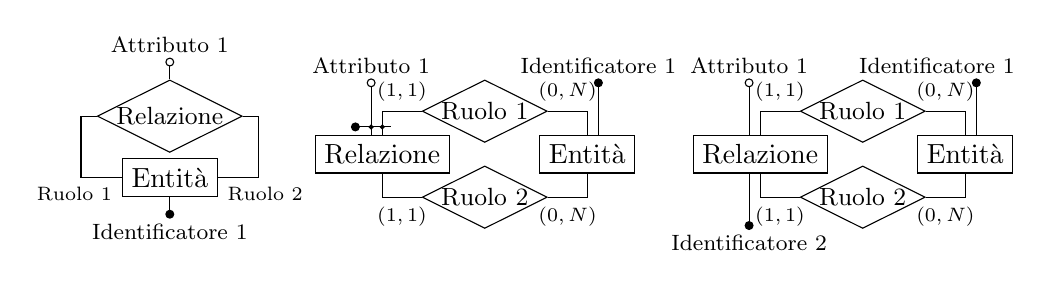
\begin{tikzpicture}
    \draw

    %%* Attributi:
    %%  node[draw, circle, inner sep=1pt, fill=black]{}node[right]{\footnotesize A}
    %%? Distanza orizzontale: E -(0.25,0.x)- A
    %%? Distanza verticale: E -(0,x * 0.22)- A

    %%* Cardinalità:
    %%  node[below right]{\scriptsize $(0,N)$}
    %%  node[above right]{\scriptsize $(0,N)$}
    %%  node[midway, above]{\scriptsize $(0,N)$}

    %%* Relazione:
    %%  node[draw, diamond, shape aspect=2, inner sep=3pt, anchor=90](r1){}
    %%  node[draw, diamond, shape aspect=2, inner sep=0.2pt, anchor=180](r2){R2}

    %%* Entità:
    %%  node[draw, rectangle, anchor=90](e1){}
    %%? Distanza verticale: E -(0.3)- R -(0.3) E
    %%? Distanza orizzontale: E -(0.75)- R -(0.75)- E
    
    (0,0)node[draw, rectangle, anchor=90](e1){Entità}
    (e1.90)++(0,1)node[draw, diamond, shape aspect=2, inner sep=0.2pt, anchor=90](r1){\small Relazione}
    (r1.0)--++(0.2,0)|-(e1.0)node[below right]{\scriptsize Ruolo 2}
    (r1.180)--++(-0.2,0)|-(e1.180)node[below left]{\scriptsize Ruolo 1}
    (r1.90)--++(0,0.22)node[draw, circle, inner sep=1pt, fill=white]{}node[above]{\footnotesize Attributo 1}
    (e1.270)--++(0,-0.22)node[draw, circle, inner sep=1pt, fill=black]{}node[below]{\footnotesize Identificatore 1}

    (r1.90)++(4,0)node[draw, diamond, shape aspect=2, inner sep=0.2pt, anchor=90](r1){\small Ruolo 1}
    (r1.0)--++(0.5,0)node[midway, above]{\scriptsize $(0,N)$}--++(0,-0.3)node[draw, rectangle, anchor=90](e1){Entità}
    (r1.180)--++(-0.5,0)node[midway, above]{\scriptsize $(1,1)$}--++(0,-0.2)node[draw, circle, inner sep=0.5pt, fill=black]{}--++(0,-0.1)node[draw, rectangle, anchor=90](e2){Relazione}
    (e1.270)--++(0,-0.3)--++(-0.5,0)node[midway, below]{\scriptsize $(0,N)$}node[draw, diamond, shape aspect=2, inner sep=0.2pt, anchor=0](r2){\small Ruolo 2}
    (r2.180)--++(-0.5,0)node[midway, below]{\scriptsize $(1,1)$}-|(e2.270)


    (e1.60)--++(0,0.66)node[draw, circle, inner sep=1pt, fill=black]{}node[above]{\footnotesize Identificatore 1}
    (e2.120)--++(0,0.1)node[draw, circle, inner sep=0.5pt, fill=black](a){}--++(0,0.56)node[draw, circle, inner sep=1pt, fill=white]{}node[above]{\footnotesize Attributo 1}
    (a)++(-0.2,0)node[draw, circle, inner sep=1pt, fill=black]{}--++(0.45,0)


    (r1.90)++(4.8,0)node[draw, diamond, shape aspect=2, inner sep=0.2pt, anchor=90](r1){\small Ruolo 1}
    (r1.0)--++(0.5,0)node[midway, above]{\scriptsize $(0,N)$}--++(0,-0.3)node[draw, rectangle, anchor=90](e1){Entità}
    (r1.180)--++(-0.5,0)node[midway, above]{\scriptsize $(1,1)$}--++(0,-0.3)node[draw, rectangle, anchor=90](e2){Relazione}
    (e1.270)--++(0,-0.3)--++(-0.5,0)node[midway, below]{\scriptsize $(0,N)$}node[draw, diamond, shape aspect=2, inner sep=0.2pt, anchor=0](r2){\small Ruolo 2}
    (r2.180)--++(-0.5,0)node[midway, below]{\scriptsize $(1,1)$}-|(e2.270)

    

    (e1.60)--++(0,0.66)node[draw, circle, inner sep=1pt, fill=black]{}++(-0.5,0)node[above]{\footnotesize Identificatore 1}
    (e2.120)--++(0,0.66)node[draw, circle, inner sep=1pt, fill=white]{}node[above]{\footnotesize Attributo 1}
    (e2.240)--++(0,-0.66)node[draw, circle, inner sep=1pt, fill=black]{}node[below]{\footnotesize Identificatore 2}
    ;
\end{tikzpicture}
\end{document}